\documentclass[12pt,a5paper]{article}
\usepackage[utf8]{inputenc}
\usepackage[russian]{babel}
\usepackage[OT1]{fontenc}
\usepackage[T1]{fontenc}
\usepackage{amsmath}
\usepackage{amsfonts}
\usepackage{amssymb}
\usepackage{makeidx}
\usepackage{graphicx}
\usepackage{colortbl}
\usepackage{multirow}
\usepackage{lmodern}
\usepackage{afterpage}
\usepackage{array}
\usepackage{physics}
\usepackage{lscape}
\usepackage{footnote}
\usepackage{threeparttable}
\usepackage[unicode, pdftex]{hyperref}
\usepackage[left=2cm,right=3cm,top=2cm,bottom=2cm]{geometry}
\usepackage{grffile}
%\usepackage{indentfirst}
%\usepackage{pdfcomment}
\renewcommand \baselinestretch{1} \normalsize
\renewcommand{\thefigure}{\thesection.\arabic{figure}}

\renewcommand{\rmdefault}{cmr} % Шрифт с засечками
\renewcommand{\sfdefault}{cmss} % Шрифт без засечек
\renewcommand{\ttdefault}{cmtt} % Моноширинный шрифт

\numberwithin{equation}{section}

\usepackage{import}
\usepackage{xifthen}
\usepackage{pdfpages}
\usepackage{transparent}
\usepackage{xcolor}
\newcommand{\incfig}[1]{%
    \def\svgwidth{\columnwidth}
    \import{./figures/}{#1.pdf_tex}
}



\begin{document}

\section{Проверка неравенства Белла}
\subsection{Введение}

Неравенства Белла (НБ) служат достаточным критерием того, что рассматриваемая система является неклассической: для классических состояний неравенства выполняются, для неклассических --- нарушаются. Поскольку НБ сконструированы на основании предположения, что существуют скрытые параметры системы, которые определяют ее состояние, то нарушение НБ квантовыми системами означает, что принципиально не существует скрытых параметров, которые бы определяли состояние системы до того, как было проведено измерение. Иными словами, нарушение неравенств Белла говорит о том, что случайность результата измерения над квантовой системой является истинной, то есть определяется фундаментальными законами природы, а не ограничением наших знаний о ней.

В данной задаче нарушение неравенств Белла будет исследовано на примере измерения поляризации пары фотонов.
% Рассмотрим состояние, представляющее собой пару поляризационно коррелированных фотонов. % в состоянии $\ket{\psi}=\ket{HH}+\ket{VV}$.
Пусть имеется два наблюдателя, Алиса и Боб, которые проводят измерения состояния поляризации, каждый над своим фотоном (рисунок упрощенной схемы). Они отправляют фотон на поляризационный светоделитель, который пропускает свет, линейно поляризованный под углом $\alpha$ (у Алисы) и $\beta$ (у Боба) к горизонтали, а ортогонально поляризованный свет отражает. В выходных каналах каждого светоделителя установлены однофототонные детекторы, и если срабатывает детектор в проходном канале, то наблюдаемая $A(\alpha)$ у Алисы и $B(\beta)$ у Боба равна $+1$, а если срабатывает детектор в отраженном канале, то соответствующая наблюдаемая равна $-1$.
% Назовем соответствующие величины переменными $A$ и $B$.


% Пусть установка (рис.~\ref{fig:Bell}) построена таким образом, что у каждого наблюдателя существует по два возможных базиса для измерений. Выбор базиса регулируется углом поворота фазовой пластинки $HWP_{A(B)}$ перед поляризационным светоделителем $PBS_{A(B)}$. Таким образом, имеется четыре линейных измерительных базиса, наклоненных относительно базиса $\{H,V\}$ на углы $\alpha$ или $\alpha'$ в канале Алисы и $\beta$ или $\beta'$ в канале Боба (углы отсчитываются в лабораторной системе координат).
%соответственно A и A$\prime$, B и B$\prime$. Для того, чтобы "переключиться" от A к A$\prime$ Алиса вращает фазовую пластинку ??, тем самым совершая переход между двумя измерительными базисами. Аналогично поступает Боб в своем канале, выбирая базис B или B$\prime$ поворотом фазовой пластины ??.


\begin{figure}[]
  \begin{center}
  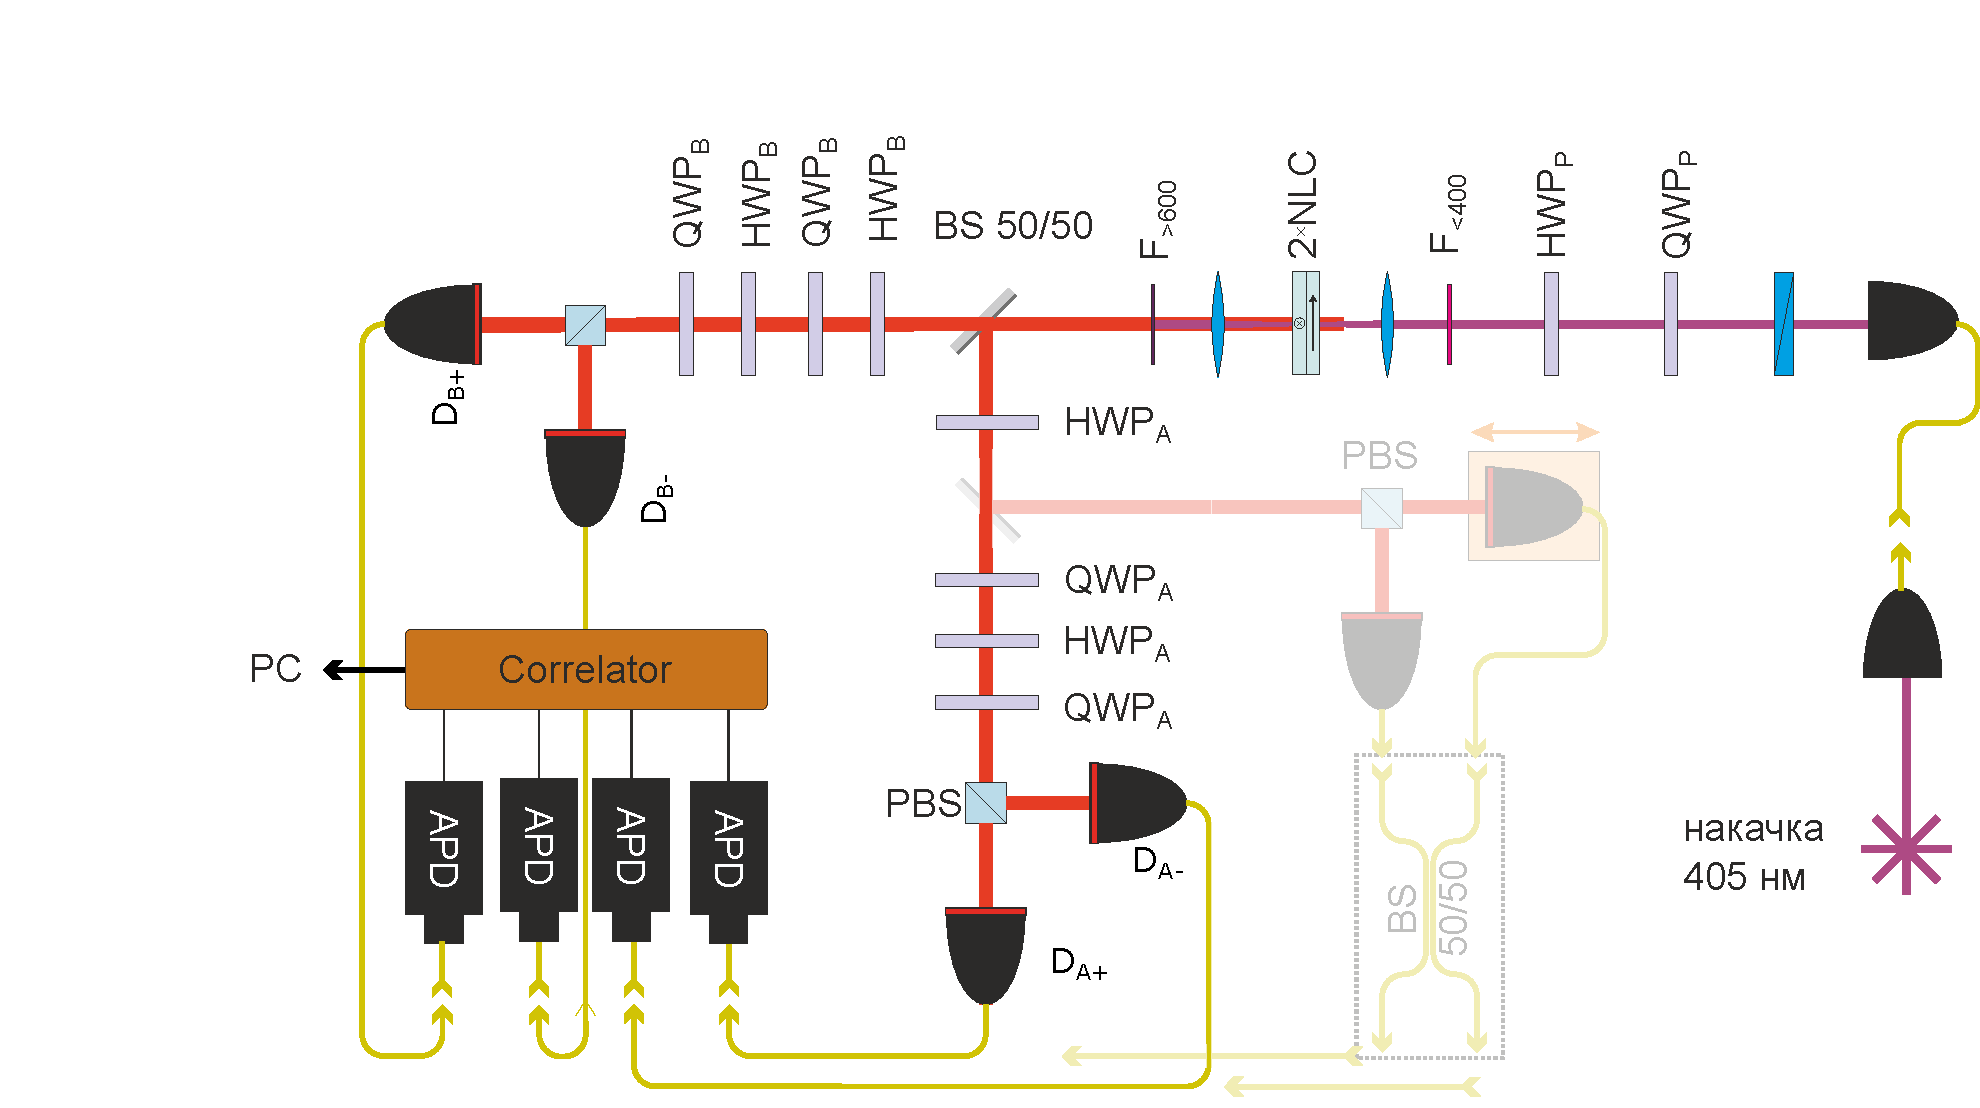
\includegraphics[width=\linewidth]{Setup_Bell_6.pdf}
  \caption{Схема установки. }\label{fig:Bell}
  \end{center}
  \end{figure}


% Примем состояние поляризации фотона равным <<+1>>, если фотон прошел через $PBS_{A(B)}$, и <<--1>>, если отразился, т.е. $A(\alpha)=\pm1$ и $B(\beta)=\pm1$, и определим среднее состояние поляризации при совместном измерении Алисой и Бобом.
%Для каждой заданной пары базисов Алисы и Боба находится среднее число совпадений $R_C$ между отсчетами  детекторов в их каналах. При этом фотоны, прошедшие через поляризационный светоделитель, учитываются в статистике совпадений со знаком <<+>>, а отраженные --- со знаком <<-->>. Таким образом,
%Величина, которую измеряет каждый наблюдатель, соответственно $A(\alpha)$ у Алисы или $B(\beta)$ у Боба, отражает то, в каком канале, прошедшем или отраженном, оказался фотон после прохождения поляризационного светоделителя. Таким образом, как $\alpha$, так и $\beta$, являются дихотомными величинами и принимают значения $\pm1$ (пусть +1 соответствует прохождению через светоделитель, а --1 --- отражению от него).
Будем посылать пары фотонов наблюдателям многократно, и каждый раз Алиса будет случайным образом выбирать одно из двух значений угла $\alpha$: $\alpha_1$ или $\alpha_2$, а, Боб, соответственно --- одно из двух значений угла $\beta$: $\beta_1$ или $\beta_2$.
Таким образом можно измерить средние значения произведений наблюдаемых $A(\alpha)B(\beta)$ для всех четырех комбинаций углов $\alpha$ и~$\beta$.

Далее рассмотрим следующую комбинацию этих средних значений:
\begin{gather}
     \left<S\right>=\left<A(\alpha_1)B(\beta_1)\right>-
     \left<A(\alpha_2)B(\beta_1)\right>+\\ \nonumber
    + \left<A(\alpha_1)B(\beta_2)\right>+
     \left<A(\alpha_2)B(\beta_1)\right>
\end{gather}
Можно рассмотреть эту комбинацию, как усредненное значение оператора $S$:
\begin{gather}
     S=A(\alpha)B(\beta)-
     A(\alpha^\prime)B(\beta)+\\ \nonumber
    + A(\alpha)B(\beta^\prime)+
     +A(\alpha^\prime)B(\beta^\prime)=\\ \nonumber
     =
     \underbrace{\left[A(\alpha)-A(\alpha^\prime)\right ]}_{0,\pm 2}
     \underbrace{B(\beta)}_{\pm 1}+
     \underbrace{\left[A(\alpha)+A(\alpha^\prime)\right]}_{\pm2,0}
     \underbrace{B(\beta^\prime)}_{\pm 1}
\end{gather}
Если предположить,что существуют скрытые параметры, которые заранее определяют результаты измерения наблюдаемых $A$, и $B$ для любых значений углов, тогда для каждого значения скрытых параметров точно определено значение наблюдаемой $S$. 
Поскольку и $A$, и $B$ принимают только значения $\pm1$, то $S$ может принимать значения только $\pm 2$, поскольку при равных значениях $A(\alpha)$ и $A(\alpha^\prime)$ первое слагаемое равно нулю, а при разных --- второе. Поскольку среднее значение наблюдаемой не может быть больше чем ее максимальное значение и меньше, чем минимальное, то будет выполняться неравенство Белла
\begin{gather}
\left|\left<S\right>\right| \le 2.
\label{S_clas2}
\end{gather}

В то же время, существуют квантовые состояния, для которых при определенных значениях $\alpha$ и $\beta$ неравенство (\ref{S_clas2}) нарушается, т.е. $\left|\left<S\right>\right| > 2$. Из этого следует вывод, что не существует совместных вероятностей результатов измерения Алисы и Боба, которые подразумеваются в рассуждении <<классическим образом>>, приведенном выше.

В данной задаче для демонстрации нарушения неравенства Белла готовится т.н. белловское состояние
\begin{gather}
\ket{\Phi_+}=(\ket{H_A H_B}+\ket{V_A V_B})/ \sqrt2,
\label{Bell_state}
\end{gather}
(индексы $A$ и $B$ отражают тот факт, что один из фотонов пары распространяется в канале Алисы, а другой --- в канале Боба), а углы фазовых пластин подбираются следующим образом:
\begin{gather}
\alpha=-\pi/8, \quad \beta=-\pi/4,\nonumber\\
\alpha^\prime=\pi/8, \quad \beta^\prime=0.
\label{alpha_beta}
\end{gather}
Рассчитаем, чему равно $\langle S \rangle$ для этого случая.

Вероятность, с которой фотон пойдет в прошедший или отраженный канал после поляризационного светоделителя у Алисы и Боба, определяется углами $\alpha$ и $\beta$. Можно показать (см. приложение \ref{app_Bell}), что среднее по состоянию $\ket{\Phi_+}$ значение результата совместного измерения
\begin{gather}
\langle A(\alpha)B(\beta) \rangle = \cos(2(\alpha-\beta)),
\label{ABquantum1}
\end{gather}
%\begin{gather}
%\langle S \rangle = \langle A(\alpha)B(\beta) \rangle - %\langle A(\alpha')B(\beta) \rangle + \nonumber \\+ \langle %A(\alpha)B(\beta') \rangle  + \langle A(\alpha')B(\beta') %\rangle,
%\label{Squantum1}
%\end{gather}
а значит, для значений углов, выбранных в соответствии с (\ref{alpha_beta}),
\begin{gather}
\langle S \rangle = 2\sqrt2,
\label{Squantum2}
\end{gather}
т.е. неравенство Белла $\langle S \rangle\leq2$ нарушается.

В эксперименте $\langle A(\alpha)B(\beta) \rangle $ измеряется как (нормированная) частота отсчетов совпадений между парой детекторов, зарегистрировавших фотоны у Алисы и Боба $R_C$. Таким образом,
\begin{gather}
\langle AB \rangle=\nonumber\\
\frac{(+1)(+1) R_C^{++} + (-1)(+1) R_C^{-+} + (+1)(-1) R_C^{+-} + (-1)(-1)R_C^{--}}{R_C^{++}+R_C^{-+}+R_C^{+-}+R_C^{--}}  \nonumber\\
=\frac{R_C^{++} - R_C^{-+} - R_C^{+-} + R_C^{--}}{R_C^{++}+R_C^{-+}+R_C^{+-}+R_C^{--}},
\label{ABquantum3}
\end{gather}
где индексы $+(-)$ соответствует случаям, когда фотон у соответствующего наблюдателя прошел (отразился) через светоделитель.

Отметим, что реальное состояние, получаемое в ходе эксперимента, может отличаться от чистого состояния $\ket{\Phi_+}$ и иметь примесь других компонент. Поэтому вычисляемая из экспериментальных данных величина $\left<S\right>$ имеет значение в диапазоне от 2 до $2\sqrt{2}$. Методика расчета $\left<S\right>$ в этом случае приведена в приложении \ref{app_S_real}.

\subsection{Юстировка}
\textit{(= Настройка HWP$_p$ и QWP$_p$ для генерации состояния $\ket{\Phi_+}$ (\ref{Bell_state}))}

\begin{itemize}
\item{Выставьте все фазовые пластинки на 0 град.}
\item{Установите HWP$_p$ под углом $45^\circ$, а затем подстройте угол таким образом, чтобы частота отсчетов в совпадениях между детекторами D$_A-$ и D$_B-$,  D$_A+$ и D$_B+$ была примерно одинакова.}
\item{Выставьте HWP$_A$ и HWP$_B$ под углом 22,5 град.}
\item{Настройте QWP$_p$ так, чтобы частота отсчетов в совпадениях между D$_A-$ и D$_B-$ была максимальной, а   частота отсчетов в совпадениях между D$_A-$ и D$_B+$ была минимальной.}
\end{itemize}

\subsection{Упражнения}
\begin{itemize}
\item{Выставьте HWP$_A$ под углом $\alpha/2=0$, пропишите зависимость всех возможных совпадений ($R_C^{++}$, $R_C^{-+}$, $R_C^{+-}$, $R_C^{--}$) от $\beta/2$  (постройте график со статистическими погрешностями).}
\item{Выставьте HWP$_A$ под углом $\alpha/2=45^\circ$, пропишите зависимость всех возможных совпадений ($R_C^{++}, R_C^{-+}, R_C^{+-}, R_C^{--}$) от $\beta/2$  (постройте график со статистическими погрешностями).}
\item{Для четырех комбинаций углов Алисы и Боба измерьте средние значения $\langle A(\alpha)B(\beta) \rangle$, $\langle A(\alpha^\prime)B(\beta) \rangle$, $\langle A(\alpha)B(\beta^\prime) \rangle$, $\langle A(\alpha^\prime)B(\beta^\prime) \rangle$ по формуле \eqref{ABquantum3}.

    Каждое измерение повторите по $N$ раз. Определите среднее значение и его статистическую погрешность.}
\item{Рассчитайте величину $\langle S \rangle$ (\ref{Squantum1}) и ее погрешность}.

    Убедитесь, что она превышает 2, и что это превышение статистически значимо.
\end{itemize}

%\textit{В зависимости от уровня сложности, можно большую или меньшую часть обработки данных включить в программу. Хорошо бы, чтобы этот уровень сложности можно было бы как-то выставить (поставить галочки в настройках). }


\subsection{Приложение 1. Расчет состояния поляризации белловского состояния}\label{app_Bell}
Состояние поляризации рассматриваемой системы математически представляет собой среднее оператора $\langle \hat{A}(\alpha) \hat{B}(\beta) \rangle$ по состоянию
$\ket\Psi=(\ket{H_A H_B}+\ket{V_A V_B})/ \sqrt2$, т.е. $\bra{\Psi}\hat{A}(\alpha) \hat{B}(\beta)\ket{\Psi}$. Операторы $A$ и $B$ действуют каждый в своем подпространстве, т.е. оператор $A(\alpha)$ действует только на фотон $A$, а оператор $B(\beta)$ --- только на фотон $B$, и представляют собой проекцию на состояния $\alpha$ и $\beta$ соответственно:

\begin{equation}
\begin{gathered}
\hat{A}(\alpha) = \ket{\alpha}_A \bra{\alpha}_A - \ket{\alpha + \pi/2}_A \bra{\alpha+\pi/2}_A \\
\hat{B}(\beta) = \ket{\beta}_B \bra{\beta}_B - \ket{\beta + \pi/2}_B \bra{\beta+\pi/2}_B.
\label{operators_Bell}
\end{gathered}
\end{equation}
Здесь $\ket{\alpha}_A = \cos \alpha \ket{H}_A + \sin \alpha \ket{V}_A$.\\
Таким образом,
\begin{equation}
\begin{gathered}
\hat{A}(\alpha) = \cos 2\alpha \big[\ket{H}_A \bra{H}_A - \ket{V}_A \bra{V}_A \big] + \\
           + \sin 2\alpha \big[\ket{H}_A \bra{V}_A + \ket{V}_A \bra{H}_A \big],
\label{operators_Bell_2}
\end{gathered}
\end{equation}
а следовательно, $ \bra{\Psi}\hat{A}(\alpha) \hat{B}(\beta)\ket{\Psi} = \cos (2\alpha - 2\beta)$.


\subsection{Приложение 2. Расчет функции $S$ для частично смешанного состояния}\label{app_S_real}
Представим матрицу генерируемого в эксперименте состояния $\rho_t$ в виде суммы матрицы чистого состояния \ref{Bell_state} $\rho_p$ и смешанного состояния $\rho_m$ с некоторым весом $p$:
\begin{gather}
\begin{split}
    &\rho_p=\frac{1}{2}\big(\ket{H}_A\ket{H}_B+\ket{V}_A\ket{V}_B\big)\big(\bra{H}_A\bra{H}_B+\bra{V}_A\bra{V}_B\big), \\
    &\rho_m=\frac{1}{2}\big(\ket{H}_A\ket{H}_B\bra{H}_A\bra{H}_B+\ket{V}_A\ket{V}_B\bra{V}_A\bra{V}_B\big), \\
    &\rho_t=p\,\rho_p+(1-p)\rho_m.
\end{split}
\label{rho_1}
\end{gather}
Подставляя $\ket{H}=\left(\begin{matrix} 1\\0 \end{matrix}\right)$ и $\ket{V}=\left(\begin{matrix} 0\\1 \end{matrix}\right)$, получим:
\begin{gather}
    \rho_t=\frac{1}{2} \left(\begin{matrix} 1&0&0&p\\0&0&0&0\\0&0&0&0\\p&0&0&1 \end{matrix}\right)
\label{rho_2}
\end{gather}
Процесс измерений одним детектором в базисе, повернутом на угол $\theta$ относительно лабораторного, описывается операторами проецирования на состояния \\ $\ket{\theta}= \cos\theta \ket{H}+\sin\theta\ket{V}$ и $\ket{\theta+\pi/2}$:
\begin{gather}
    \hat{A}({\theta})=\ket{\theta}\bra{\theta}-\ket{\theta+\pi/2}\bra{\theta+\pi/2}
\label{A}
\end{gather}
Измерение двумя детекторами в базисах $\theta_1$ и $\theta_2$, таким образом,-- это тензорное произведение операторов $\hat{A}_A({\theta_1})\hat{A}_B({\theta_2})$.
Когда оба детектора проводят измерения в диагональном базисе (для антидиагонального ответ будет тем же),
\begin{gather}
    I_{max}=\mbox{Tr}\left\{\frac{1}{2} \frac{1}{4}
    \left(\begin{matrix} 1&0&0&p\\0&0&0&0\\0&0&0&0\\p&0&0&1 \end{matrix}\right)
    \left(\begin{matrix} 1&1&1&1\\1&1&1&1\\1&1&1&1\\1&1&1&1 \end{matrix}\right)\right\}=
    \frac{1+p}{4},
\label{I_max}
\end{gather}
Аналогично можно получить, что когда один детектор производит измерения в диагональном базисе, а второй -- в антидиагональном, $I_{min} = (1-p)/4$. Для полностью чистого состояния $p=1$, и $I_{min} = 0$, для полностью смешанного $p=0$, и $I_{min} = I_{max}$.

Таким образом, долю чистого состояния в смеси можно вычислить из соотношения измеренных в эксперименте величин $I_{max}$ и $I_{min}$ и равенства
\begin{gather}
    \frac{1+p}{1-p}=\frac{I_{max}}{I_{min}},
\label{p_exp}
\end{gather}
Белловские измерения проводятся аналогично:
\begin{gather}
    \langle A(\alpha)B(\beta) \rangle = \mbox{Tr}\left\{\rho_t\hat{A}_A(\alpha)\hat{A}_B(\beta)\right\}.
\label{AB}
\end{gather}


\section{Провал Манделя}
\subsection{Введение}

В данной задаче изучается интерференция двух фотонов на светоделителе, которая позволяет измерять ширину спектра двухфотонного излучения с высокой точностью. Впервые эффект был продемонстрирован в работе \cite{Hong1987}, и впоследствии назван в честь одного из авторов. Идея эксперимента (рис.~\ref{fig:HOM_paper}(а)) состояла в следующем.

\begin{figure}[]
  \begin{center}
  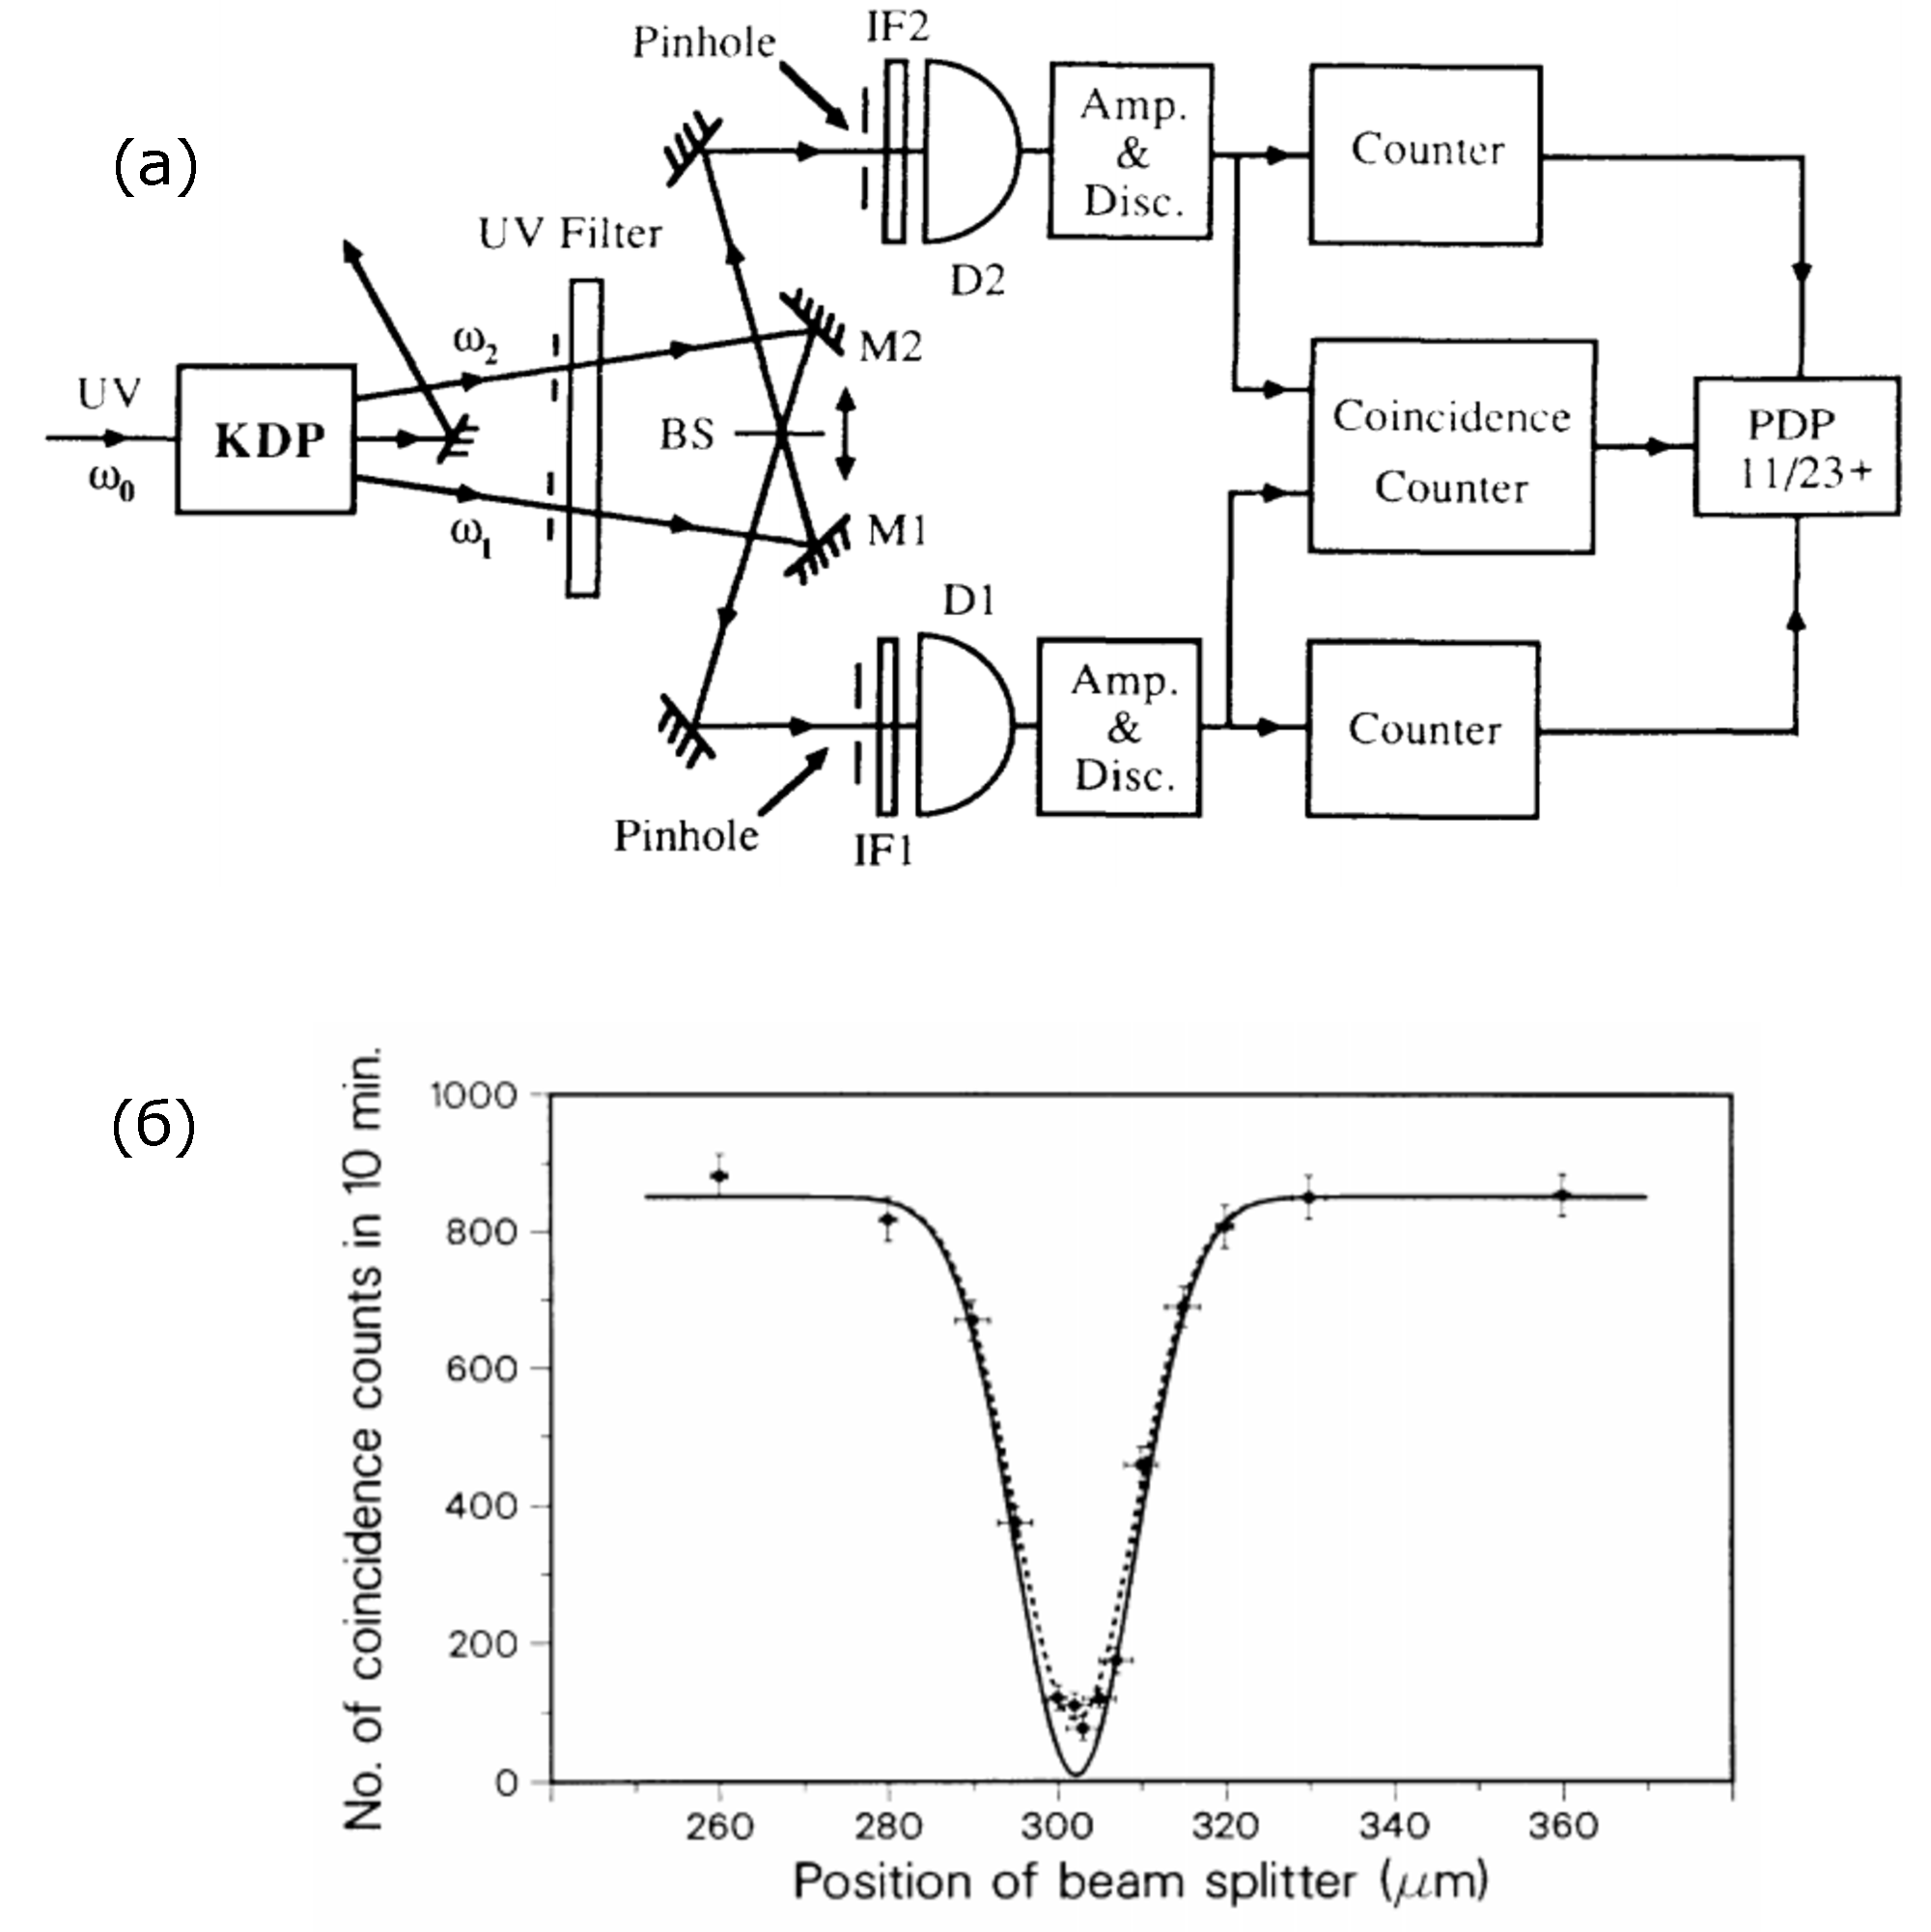
\includegraphics[width=\linewidth]{HOM_paper3.pdf}
  \caption{(а) Схема установки из работы \cite{Hong1987} и (б) "провал" в скорости регистрации совпадений между детекторами D1 и D2, достигаемый при равенстве оптических путей обоих фотонов. }\label{fig:HOM_paper}
  \end{center}
  \end{figure}

Пары фотонов генерировались в процессе спонтанного параметрического рассеяния (СПР). Поскольку генерация происходила в неколлинеарном вырожденном режиме, фотоны внутри каждой пары распространялись после кристалла в разных направлениях. Далее они сбивались на неполяризационном светоделителе, после чего с равной вероятностью либо отражались, либо проходили через него, и регистрировались детекторами. Сигналы с обоих детекторов сравнивались и подсчитывалось количество совпадений между ними внутри малого временного окна в зависимости от положения светоделителя, т.е. от разницы длин оптический путей каждого фотона от кристалла до светоделителя (рис. \ref{fig:HOM_paper}(б)).

При точном совпадении оптических путей оба фотона после светоделителя с единичной вероятностью попадают в один и тот же канал, что отражается на графике \ref{fig:HOM_paper}(б) падением числа совпадений до нуля. Ширина провала определяет ширину спектра исследуемого двухфотонного излучения.

Пусть в процессе СПР в кристалле родились два фотона с частотами $\omega_1$ и $\omega_2$, и после кристалла они вылетели в направлениях $\theta_1$ и $\theta_2$. Состояние двухфотонного поля в таком случае можно описать действием операторов рождения в модах \{$\omega_1, \theta_1$\} и \{$\omega_2, \theta_2$\}:
\begin{gather}
    \ket{\psi^{in}}=\phi(\omega_1, \omega_2)a^{\dagger}(\omega_1, \theta_1) a^{\dagger}(\omega_2, \theta_2)\ket{0},  \label{psi_in_1}
 \end{gather}
с коэффициентом пропорциональности $\phi(\omega_1, \omega_2)$, называемым амплитудой двухфотонного поля.

Операторы уничтожения во входных модах светоделителя $in_{1,2}$ (рис.~\ref{fig:BS}) преобразуются в операторы уничтожения в выходных модах $out_{1,2}$ в соответствии с матрицей
\begin{gather}
   \begin{pmatrix}
    a^{out}_1 \\ a^{out}_2
   \end{pmatrix} =
    \begin{pmatrix}
        \sqrt{R} & i\sqrt{T} \\
        i\sqrt{T} & \sqrt{R}
    \end{pmatrix}
   \begin{pmatrix}
    a^{in}_1 \\ a^{in}_2
   \end{pmatrix} \label{BS_matrix}
\end{gather}


\begin{figure}[]
    \centering
    \incfig{BS_4}
    \caption{К пояснению обозначений в тексте.}
    \label{fig:BS}
\end{figure}

%\begin{figure}[]
%  \begin{center}
%  \import{./figures/}{BS_2.pdf_tex}
%  \caption{К пояснению обозначений в тексте.}\label{fig:BS}
%  \end{center}
%  \end{figure}

Поскольку фотоны, вылетающие под разными направлениями из кристалла, попадают на разные входы светоделителя, \ref{psi_in_1} можно переписать в виде
\begin{gather}
    \ket{\psi^{in}}\propto a^{ in}_1 (\omega_1) ^ \dagger a^{in}_2 (\omega_2) ^ \dagger\ket{0}\equiv\ket{1,1}, \label{psi_in_2}
\end{gather}
и с учетом \ref{BS_matrix}, состояние поля на выходе светоделителя имеет вид
\begin{gather}
    \ket{\psi^{out}}\propto (R-T)\ket{1,1} + i\sqrt{2RT} (\ket{2,0}+\ket{0,2})
     \label{psi_out}
\end{gather}

Можно заметить, что при равенстве коэффициентов пропускания и отражения светоделителя в выходном излучении не будет фотонов в состоянии $\ket{1,1}$, т.е. в каждой паре оба фотона попадут в один и тот же канал.

\subsection{Экспериментальная установка}
Экспериментальная установка, которая реализована в данной задаче (рис. \ref{fig:Setup_HOM}), несколько отличается от предложенной Хонгом, Оу и Манделем.

\begin{figure}[h]
  \begin{center}
  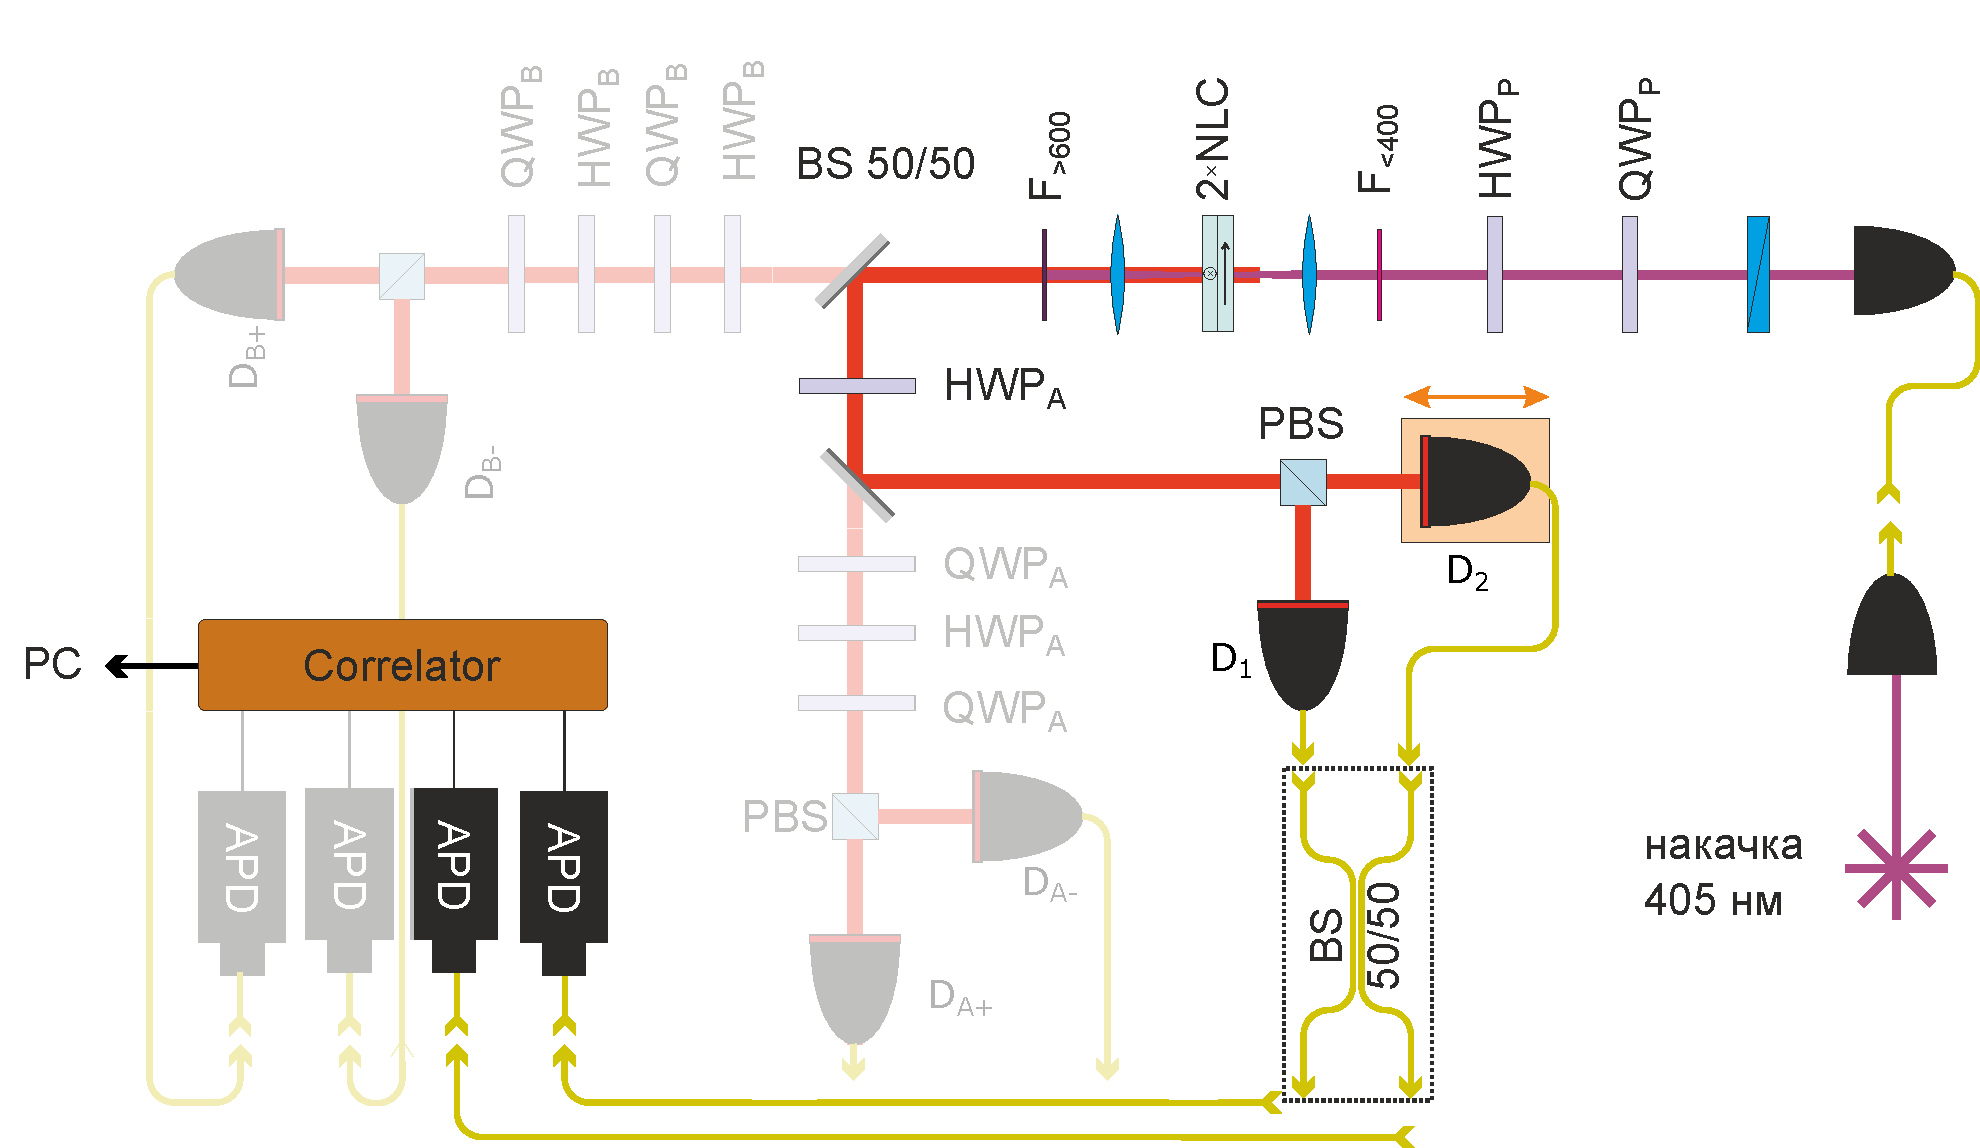
\includegraphics[width=\linewidth]{Setup_HOM_4.pdf}
  \caption{Схема установки. }\label{fig:Setup_HOM}
  \end{center}
  \end{figure}

Изначально источником фотонов служит излучение спонтанного параметрического рассеяния, генерируемое в паре нелинейных кристаллов 2$\times$NLC в состоянии $(\ket{HH} - \ket{VV})/\sqrt{2}$. После симметричного неполяризационного светоделителя BS 50/50 с вероятностью 1/4 оба фотона из каждой пары отражаются в канал А, с вероятностью 1/4 оба фотона проходят в канал В и с вероятностью 1/2 по одному фотону оказывается в отраженном и прошедшем каналах.  Нас будут интересовать только те пары, в которых оба фотона попали в отраженный канал.

Для пространственного разделения фотонов по двум входам волоконного светоделителя используется поляризационный светоделитель PBS$_C$ в комбинации с полуволновой пластиной HWP$_A$, установленной под углом $22,5^\circ$. В результате светоделитель разделяет фотоны, которые до преобразования полуволновой пластиной имели диагональную и антидиагональную поляризацию (а после --- вертикальную и горизонтальную). Можно показать, что запись $(\ket{HH} - \ket{VV})/\sqrt{2}$ в <<горизонтальном>> базисе \{H,V\} эквивалентна записи $(\ket{AD} + \ket{DA})/\sqrt{2}$ в <<диагональном>> базисе \{D,A\}. Таким образом, в каждой паре один из фотонов отражается от светоделителя, а второй проходит через него, попадая в дальнейшем на разные входы волоконного светоделителя.

Для того, чтобы была возможна интерференция, излучение фокусируется в поляризационно сохраняющее волокно, и фотоны из разных каналов распространяются в ортогонально поляризованных модах.


Можно показать (см. приложение~\ref{bandwidth_calculation}), что форма провала Манделя, т.е. зависимость числа совпадений от временной задержки $\tau$ между фотонами в момент попадания на светоделитель (рис.~\ref{fig:HOM_paper}(б)) определяется шириной спектра исследуемого двухфотонного поля и при $T=R$ имеет вид
\begin{gather}
 P\propto 1-\exp^{-(\Delta\omega \tau)^2/4}.\label{P_2}
\end{gather}
 Поэтому в ходе выполнения работы предлагается сравнить указанные зависимости для полей с разной шириной, которая фиксирована спектрами пропускания фильтров, установленных в каплерах $D_1$ и $D_2$.

\subsection{Юстировка}
1. Выставьте HWP$_p$ так, чтобы генерировалось состояние $(\ket{HH} - \ket{VV})/\sqrt{2}$.\\
2. Проверьте с помощью линейки, что длина оптических путей фотонов между поляризационным светоделителем и каплерами $D_1$ и $D_2$ одинакова. (?)


\subsection{Упражнения}
1. Установите на оба каплера $D_1$ и $D_2$ фильтры <<810(10)>>. Проведите измерение числа совпадений детекторов, сканируя положение каплера $D_2$ трансляционной подвижкой.\\
2. Повторите эксперимент, заменив в обоих каплерах фильтры <<810(10)>> на фильтры <<800(40)>> (спектры пропускания фильтров приведены в приложении~\ref{filters_spectra}).\\
Из экспериментальных данных вычислите ширину спектра двухфотонного поля, используя формулы \ref{P_2}  и  \ref{P}.


\subsection{Приложение 1. Расчет ширины провала Манделя} \label{bandwidth_calculation}

Пусть один из детекторов регистрирует фотон с частотой $\omega_3$ в момент времени $t_3$, а второй --- фотон с частотой $\omega_4$ в момент времени $t_4$.
Математически этот процесс представляет собой проецирование состояния \ref{psi_in_1} на состояние
\begin{gather}
    \ket{\psi_M}\propto \int d\omega_3 d\omega_4 \left(a_1^{out}(\omega_3) \right)^\dagger \left(a_2^{out}(\omega_4)\right)^\dagger
    e^{-i\omega_3 t_3} e^{-i\omega_4 t_4} \ket{0}, \label{psi_M}
 \end{gather}
 после прохождения фотонами расстояния от светоделителя до детектора за времена $t_3$ и $t_4$.

Число совпадений между детекторами равно $|\bra{\psi_M}\ket{\psi^{in}}|^2$. Учитывая \ref{BS_matrix}, а также
\begin{equation}
\begin{split}
    &a_1^{in}(\omega_3)a_1^{in}(\omega_4)\left(a_1^{in}(\omega_1) \right)^\dagger \left(a_2^{in}(\omega_2)\right)^\dagger \ket{0} =0, \nonumber\\
    &a_2^{in}(\omega_3)a_1^{in}(\omega_4)\left(a_1^{in}(\omega_1) \right)^\dagger \left(a_2^{in}(\omega_2)\right)^\dagger \ket{0} =\delta(\omega_1-\omega_4) \delta(\omega_2-\omega_3), \nonumber\\
    &a_1^{in}(\omega_3)a_2^{in}(\omega_4)\left(a_1^{in}(\omega_1) \right)^\dagger \left(a_2^{in}(\omega_2)\right)^\dagger \ket{0} =\delta(\omega_1-\omega_3) \delta(\omega_2-\omega_4), \nonumber\\
    &a_2^{in}(\omega_3)a_2^{in}(\omega_4)\left(a_1^{in}(\omega_1) \right)^\dagger \left(a_2^{in}(\omega_2)\right)^\dagger \ket{0} =0,
\label{aax}
\end{split}
\end{equation}
получим
\begin{equation}
\begin{split}
    \bra{\psi_M}\ket{\psi^{in}}& \propto  \int d\omega_1 d\omega_2 d\omega_3 d\omega_4 \phi(\omega_1,\omega_2)
    (R \delta(\omega_1-\omega_3) \delta(\omega_2-\omega_4)- \\
    &-T \delta(\omega_1-\omega_4) \delta(\omega_2-\omega_3))
    e^{i\omega_3 t_3} e^{i\omega_4 t_4}= \\
    &= \int d\omega_1 d\omega_2 (R\phi(\omega_3,\omega_4-T\phi(\omega_4,\omega_3))
    e^{i\omega_3 t_3} e^{i\omega_4 t_4}
\label{FT}
\end{split}
\end{equation}

Для пар фотонов, рожденных в процессе СПР, выполняется соотношение $\omega_1+\omega_2=\omega_p$, где $\omega_p$- частота накачки, причем частоты обоих фотонов распределены вокруг центральной частоты $\omega_p/2$. Кроме того, сделаем замену $t_3=\tau$, $t_4=\tau-\delta\tau$, где $\delta\tau$ обозначает разность хода фотонов по времени. Тогда \ref{FT} преобразуется к виду
\begin{equation}
\begin{split}
    \bra{\psi_M}\ket{\psi^{in}}& \propto R G(\tau)-TG^*(\delta\tau-\tau),
\label{FT2}
\end{split}
\end{equation}
где $G(\tau)\propto \int d\omega \phi(\omega_p/2+\omega, \omega_p/2-\omega) e^{-i\omega\tau}$ --- корреляционная функция исследуемого излучения.

Следовательно, вероятность зарегистрировать совпадения между детекторами равна \begin{equation}
\begin{split}
    P\equiv|\bra{\psi_M}\ket{\psi^{in}}|^2 \propto &
     R^2 |G(\tau)|^2+T^2 |G(\delta\tau-\tau)|^2 -\\
     &-RT (G(\tau)G^*(\delta\tau-\tau)+ c.c.),
\label{CC_1}
\end{split}
\end{equation}

Далее необходимо учесть, что время усреднения при регистрации совпадений много меньше времени когерентности поля, поэтому выражение \ref{CC_1} должно быть проинтегрировано по $\tau$ в бесконечных пределах. При этом если $\delta\tau$ больше времени когерентности, то последнее слагаемое будет равно нулю, т.е. $P=R+T=1$, а если $\delta\tau=0$, т. е. длина оптических путей фотонов одинакова, то $P=(R-T)^2$, и число совпадений равно нулю при $R=T$.

Амплитуду двухфотонного поля  принято представлять в гауссовом приближении \begin{gather}
   \phi(\omega_1, \omega_2) \propto \exp{-\frac{(\omega_1-\omega_2)^2}{2\Delta\omega^2}}, \label{phi}
 \end{gather}
а поскольку $G(\tau)$ представляет собой результат преобразования Фурье от $\phi(\omega_1, \omega_2)$, то она тоже имеет гауссову форму
$G(\tau)\propto \exp{-\tau^2 \Delta\omega^2/2}$.
Подстановкой в \ref{CC_1} можно получить искомую зависимость
\begin{gather}
    P\propto 1-\frac{2RT}{R^2+T^2} e^{-(\Delta\omega \delta\tau)^2/4}. \label{P}
 \end{gather}


\subsection{Приложение 2. Спектры пропускания фильтров} \label{filters_spectra}
\begin{figure}[]
  \begin{center}
  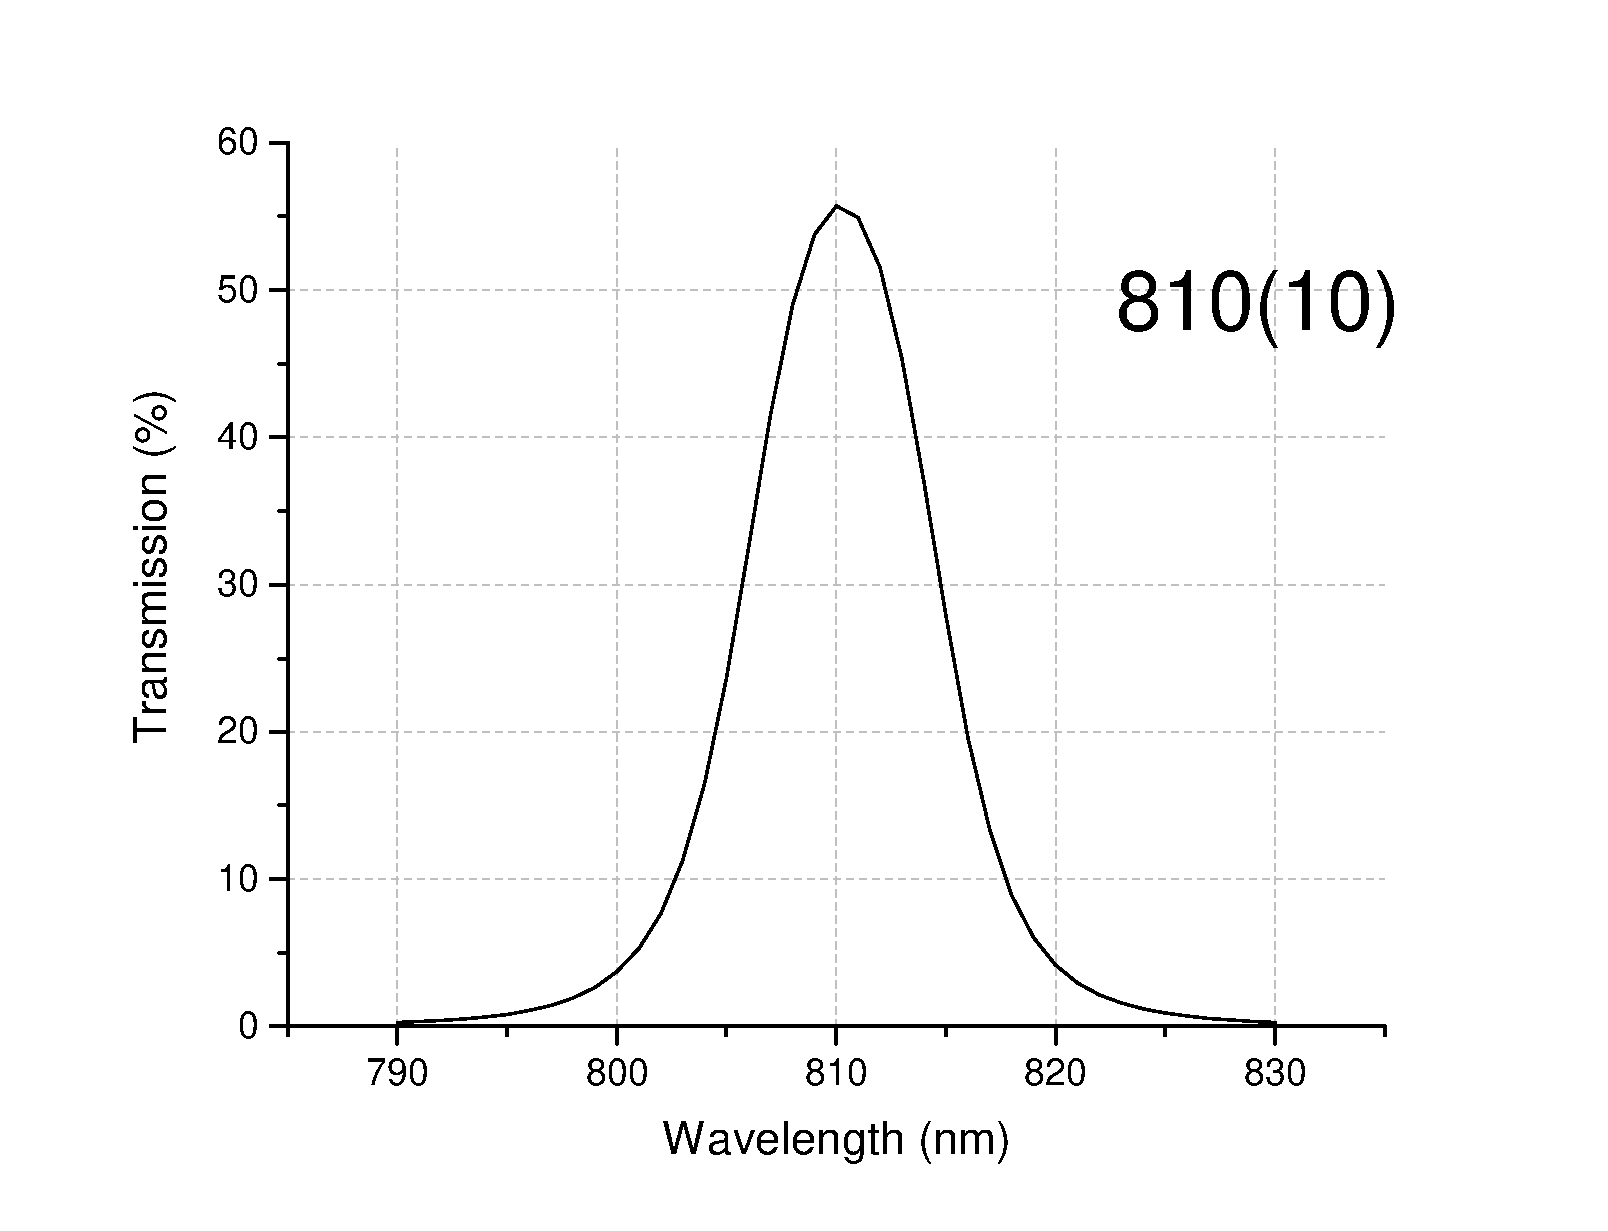
\includegraphics[width=\linewidth]{filters_spectra/810_10.pdf}
  \caption{Спектр пропускания фильтра <<810(10)>>. }\label{fig:810(10)}
  \end{center}
  \end{figure}

\begin{figure}[]
  \begin{center}
  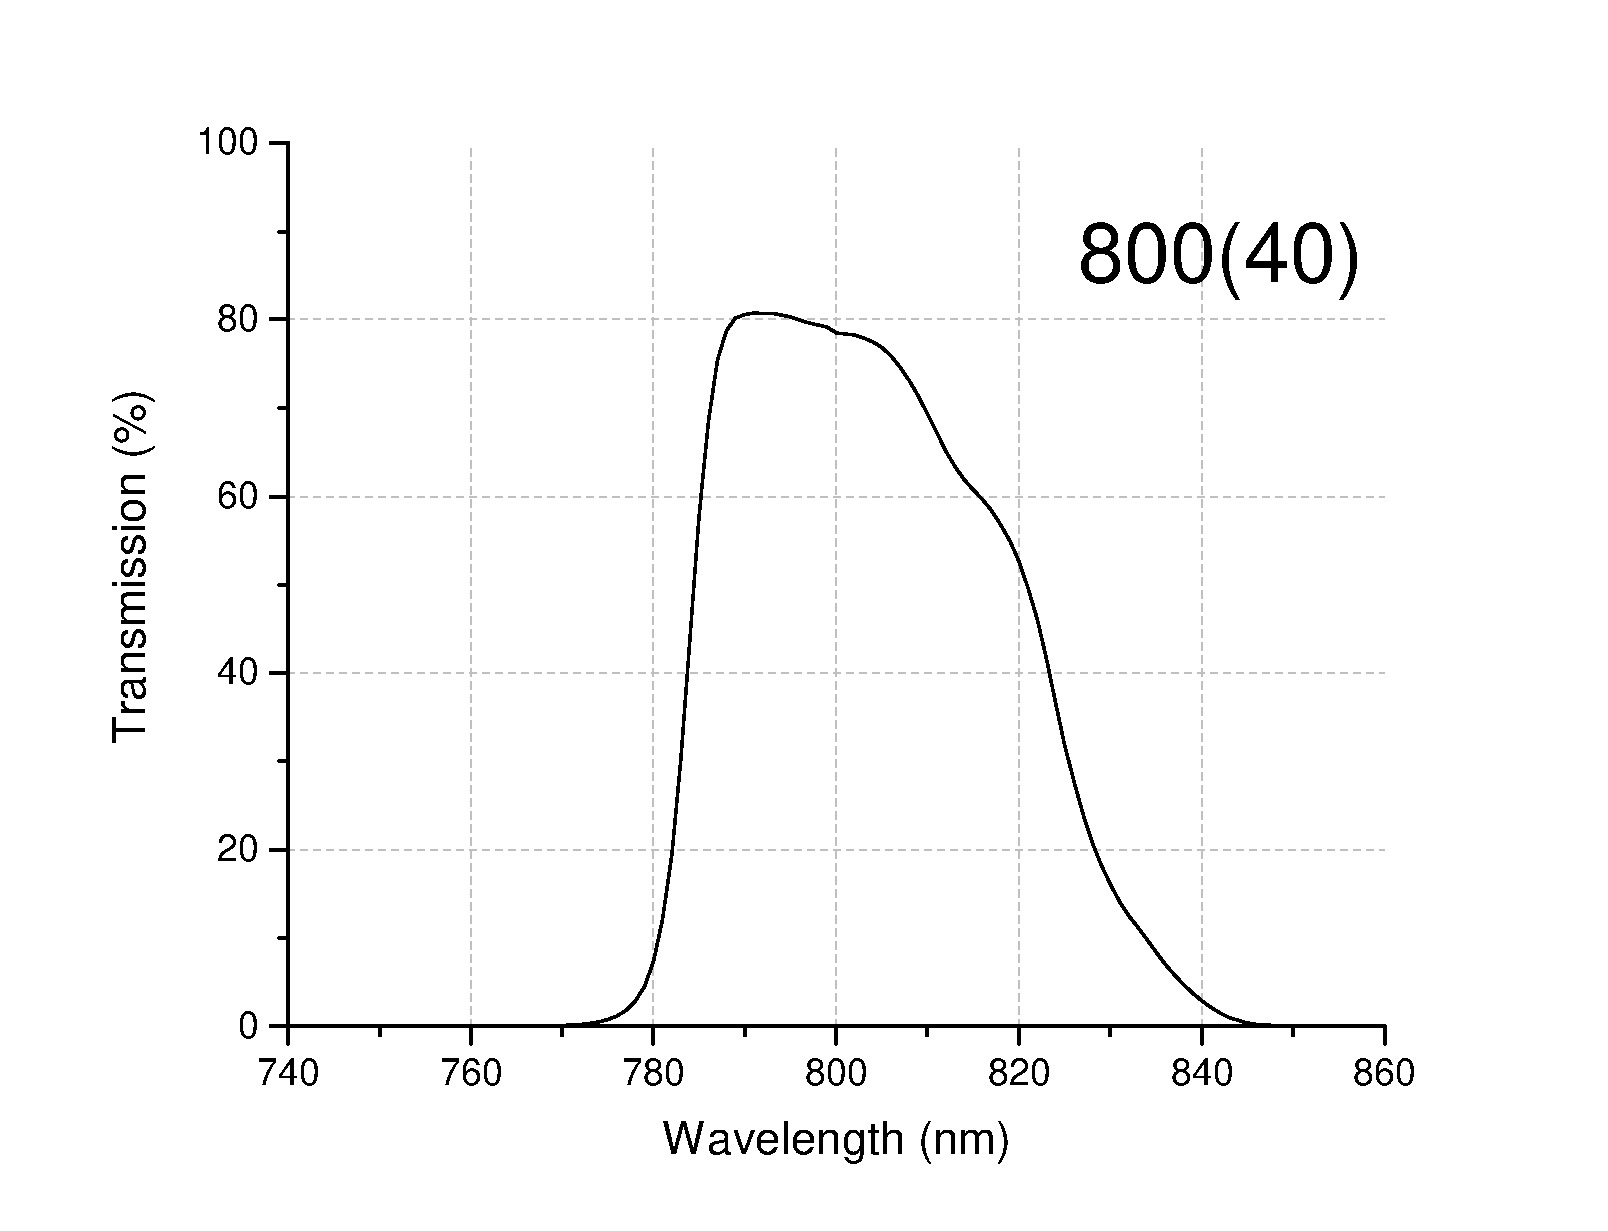
\includegraphics[width=\linewidth]{filters_spectra/800_40_2.pdf}
  \caption{Спектр пропускания фильтра <<800(40)>>. }\label{fig:800(40)}
  \end{center}
  \end{figure}


\newpage
\section{\refname}
\renewcommand{\refname}{}
\bibliographystyle{gost780u}
\bibliography{library22082019}
\end{document}
